\documentclass[8pt,pdf,hyperref={unicode}]{beamer}
% \documentclass[aspectratio=43]{beamer}
% \documentclass[aspectratio=1610]{beamer}
% \documentclass[aspectratio=169]{beamer}
\usepackage{lmodern}
\usepackage{amsfonts}
\usepackage{amsmath}
% тема оформления
%\usetheme{CambridgeUS}
%Закругление выделений
%\useinnertheme{rounded}
%Настройка темы самого слайда
%\useoutertheme{infolines}
%\useoutertheme[subsection=true, footline=authortitle]{miniframes}
\usetheme{Boadilla}
\useoutertheme[subsection=true, footline=authortitle]{miniframes}
\makeatother
\setbeamertemplate{footline}
{
    \leavevmode%
    \hbox{%
        \begin{beamercolorbox}[wd=.4\paperwidth,ht=2.25ex,dp=1ex,center]{author in head/foot}%
            \usebeamerfont{author in head/foot}\insertshortauthor
        \end{beamercolorbox}%
        \begin{beamercolorbox}[wd=.6\paperwidth,ht=2.25ex,dp=1ex,center]{title in head/foot}%
            \usebeamerfont{title in head/foot}\insertshorttitle\hspace*{3em}
            \insertframenumber{} / \inserttotalframenumber\hspace*{1ex}
        \end{beamercolorbox}}%
        \vskip0pt%
    }
\makeatletter
% отключить клавиши навигации
\setbeamertemplate{navigation symbols}{}
% цветовая схема
\usecolortheme{spruce}


\title{Turchin's method of statistical regularization}   
%\subtitle{Overview report}
\author{\underline{Mikhail Zelenyi} \inst{1,2} \and Maria Polyakova(Nelyubina)\inst{1,2}}
\institute[INR]{
    \inst{1} Institute for Nuclear Research RAS \and
    \inst{2} Moscow Institute of Physics and Technology
    }
\date{\today}

%\logo{\includegraphics[height=5mm]{image/logo.png}\vspace{-7pt}}

\begin{document}
    % титульный слайд
    \begin{frame}
        \titlepage
    \end{frame}
    
\begin{frame}
  \begin{block}{Scheme of an experiment}
      
  
    \begin{columns}
        \begin{column}{0.15\textwidth}
            \includegraphics[width=\textwidth]{image/data512.png}\\
        \end{column}
        \begin{column}{0.05\textwidth}
            \includegraphics[width=1\textwidth]{image/equtation.jpeg}
        \end{column}
        \begin{column}{0.15\textwidth}
            \includegraphics[width=1\textwidth]{image/search.png}\\
        \end{column}
        \begin{column}{0.05\textwidth}
            \includegraphics[width=1\textwidth]{image/plus.jpeg}
        \end{column}
        \begin{column}{0.15\textwidth}
            \includegraphics[width=1\textwidth]{image/pribor.png}\\
        \end{column}
        \begin{column}{0.05\textwidth} 
            \includegraphics[width=1\textwidth]{image/plus.jpeg}
        \end{column}
        \begin{column}{0.15\textwidth} 
            \includegraphics[width=1\textwidth]{image/oscillator_noise.png}\\
        \end{column}
    \end{columns}
~~~~\\~~~\\    
    \begin{columns}
        \begin{column}{0.15\textwidth}
            \LARGE{Experimental data}
        \end{column}
        \begin{column}{0.05\textwidth}
        \end{column}
        \begin{column}{0.15\textwidth}
            \LARGE{Observed value}
        \end{column}
        \begin{column}{0.05\textwidth}
        \end{column}
        \begin{column}{0.15\textwidth}
            \LARGE{Apparatus function}
        \end{column}
        \begin{column}{0.05\textwidth} 
        \end{column}
        \begin{column}{0.15\textwidth} 
            \LARGE{A bit of noise}
        \end{column}
    \end{columns}

~~~~\\

    \begin{columns}
        \begin{column}{0.15\textwidth}
            \LARGE{
                $$
                f(y)
                $$
                }
        \end{column}
        \begin{column}{0.05\textwidth}
                \LARGE{
                    $$
                    =
                    $$
                }
        \end{column}
        \begin{column}{0.15\textwidth}
            \LARGE{
                $$
                \varphi(x)
                $$}
        \end{column}
        \begin{column}{0.05\textwidth}
                            \LARGE{
                                $$
                                \ast
                                $$
                            }
        \end{column}
        \begin{column}{0.15\textwidth}
                        \LARGE{
                            $$
                            K(x,y)
                            $$}
        \end{column}
        \begin{column}{0.05\textwidth}
                            \LARGE{
                                $$
                                +
                                $$
                            }
        \end{column}
        \begin{column}{0.15\textwidth} 
                           \LARGE{
                               $$
                               \varepsilon_y
                               $$
                            }
        \end{column}
    \end{columns}
     \end{block}
     
     \begin{block}{Processing: Solution of Fredholm integral equation}
         \begin{columns}
             \column{0.15\textwidth}
             \includegraphics[width=\textwidth]{image/data512.png}
             \column{0.1\textwidth}
             \includegraphics[width=\textwidth]{image/next_318-140722.jpg}                            
             \column{0.15\textwidth}
             \includegraphics[width=\textwidth]{image/batch_processing.png}
             \column{0.05\textwidth}
             \Huge{:}
             \column{0.5\textwidth}
             \LARGE{
                 $$
                 f(y) = \int dx~ K(x,y)\varphi(x)
                 $$
                 $$
                 \varphi(x) - ?
                 $$
                } 
         \end{columns}
        \end{block}
\end{frame}


\begin{frame}
    %2 slide
    \frametitle{Solution of Fredholm equation (least squares)}
    \begin{columns}[c]
        \begin{column}{0.45\textwidth}
            {\LARGE
                In the integral form:
                $$
                f(y) = \int dx~ K(x,y)\varphi(x)
                $$
                For transition to matrix form:
                $$
                \varphi(x) = \sum \limits_n \varphi_n T_n(x),
                $$
                where $\left\lbrace T_n(x)\right\rbrace $ is some function basis.

    }
\end{column}
%        \hspace{-50pt}
        \vrule{}
         \hspace{5pt}
     \begin{column}{0.45\textwidth}
                {\LARGE
                Then:
                $$
                K_{mn} = \int K(x,y_m)T_n(x)~dx
                $$
                $$
                f_m = f(y_m)
                $$
                In the matrix form:
                $$
                f_m = K_{mn}\varphi_n
                $$
                Solution with using method of least squares:
                $$
                \varphi_n = (K_{mn}^{T}K_{mn})^{-1}K_{mn}^{T}f_m
                $$
                    
                }
            
\end{column}

    \end{columns}
    \end{frame}
\begin{frame}
   \frametitle{Numerical simulation: generation of data}
   \begin{columns}
       \column{0.45\textwidth}
       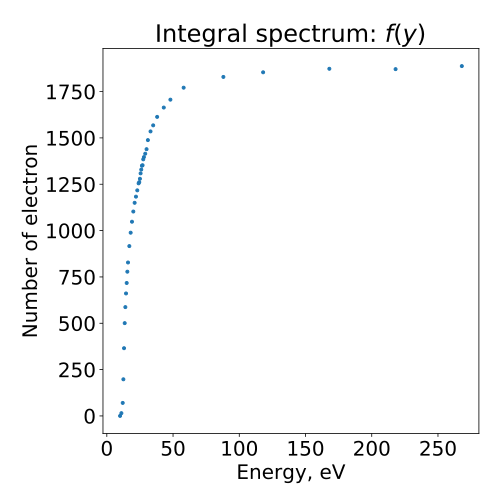
\includegraphics[width=1\textwidth]{image/fig01.png}\\
       \includegraphics[width=1\textwidth]{image/fig03.png}
       \column{0.45\textwidth}
       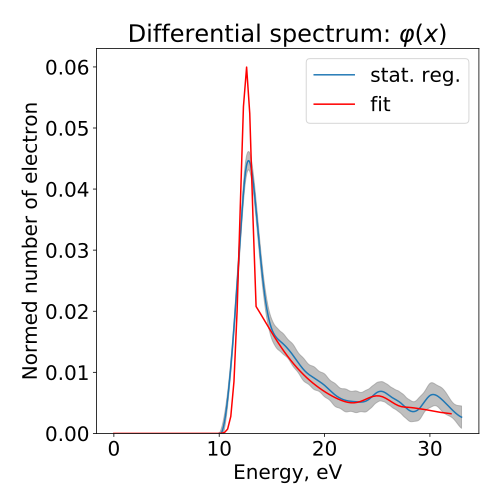
\includegraphics[width=1\textwidth]{image/fig02.png}\\
       \includegraphics[width=1\textwidth]{image/fig04.png}
    \end{columns}
\end{frame}


\begin{frame}
    \frametitle{Numerical simulation: comparison of two methods}
 \begin{center}
        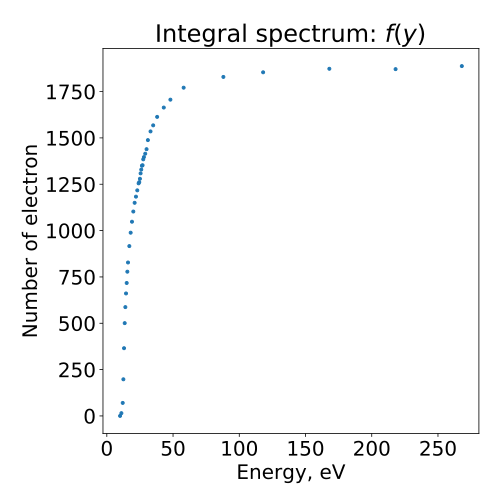
\includegraphics[width=0.4\textwidth, height=0.4\textheight]{image/fig01.png}
    \end{center}
    \begin{columns}
        \column{0.45\textwidth}
        \includegraphics[width=1\textwidth]{image/fig05.png}
        \column{0.45\textwidth}
        \includegraphics[width=1\textwidth]{image/fig06.png}
    \end{columns}
\end{frame}

\begin{frame}
    \frametitle{}
    
    \begin{block}{Problem.}
        \begin{columns}[c]
            \begin{column}{0.45\textwidth}
            
            {\LARGE
                In the integral form:
                $$
                f(y) = \int dx~ K(x,y)\varphi(x).
                $$
                Fredholm equation is ill-possed.
            }
        \end{column}
                    \vrule{}
                    \hspace{5pt}
            \begin{column}{0.45\textwidth}        
            {\LARGE
                In the matrix form:       
                $$
                f_m = K_{mn}\varphi_n
                $$
                Matrix $K$ is ill-conditioned
            }
        \end{column}
        \end{columns}
     \end{block}
     \begin{block}{In summary}
 \begin{center}
        {\LARGE A small error when measuring $f(y)$ leads to big instability of $\varphi(x)$.}
    \end{center}
\end{block}

     \begin{block}{Alternative solution --- to use regularization}
\begin{center}
             {\LARGE \textbf{Regularization} is a process of introducing additional information for transition from ill-possed problem to well-possed problem.}
\end{center}
        \end{block}
\end{frame}





\begin{frame}[squeeze]
    \frametitle{Turchin's method of statistical regularization }
    \begin{block}{Main features}
    {\LARGE     \begin{itemize}
        \item Based on Bayesian approach and decision theory (choice theory)\\
        \item Considered different a prior information: smoothness, non-negatives. \\
        \item Defined errors of obtained solution!\\
        \item Don't contend undefined parameter\\
    \end{itemize}}
    \end{block}
    \begin{block}{Description}
{\LARGE         Choice of solution based on strategy $\hat{S}$, which used a prior information.
        $$
        Optimal~ \varphi(x) = \hat{S}[f] = E[\varphi|f] = \int \varphi  \frac{P(\varphi)P(f|\varphi)}{Norm}d\varphi
        $$
        Error of solution:
        $$
        D(x_1,x_2)  = E[\varphi(x_1) - \hat{S}[f](x_1)][\varphi(x_2) - \hat{S}[f](x_2)]
        $$}
    \end{block}
\end{frame}

\begin{frame}
    \frametitle{Turchin's method of statistical regularization}
{\LARGE     Choice based on strategy $\hat{S}[f]$.\\
    Good strategy minimize wrong from our ignorance.\\
    Our ignorance is defined loss-function:
    $$
    L(\varphi,\hat{S}[f]) = ||\varphi-\hat{S}[f])||_{L_2},
    $$
    For this loss-function:
    $$
    \hat{S}[f] = E[\varphi|f] = \int \varphi P(\varphi|f)d\varphi
    \label{eq:opt}
    $$
    Strategy depend on prior information $P(\varphi)$:
    $$
    P(\varphi|f)= \frac{P(\varphi)P(f|\varphi)}{\int d\varphi P(\varphi)P(f|\varphi)} 
    $$
    Error of solution:
    $$
    D(x_1,x_2)  = E[\varphi(x_1) - \hat{S}[f](x_1)][\varphi(x_2) - \hat{S}[f](x_2)]
    $$}
    
\end{frame}


\begin{frame}
    \frametitle{A prior information (smoothness)}

\only<1>{\begin{block}{Condition on prior information}
{\LARGE                
    Limit Shannon's information in prior probability:
    $$
    I[P(\varphi)] = \int \ln{P(\varphi)} P(\varphi) d\varphi \to min
    $$
    Normalize:
    $$
    \int P(\varphi) d\varphi = 1
    $$    
    Choose more smoothness solutions:
    $$
    \int \langle \varphi,\hat{\Omega}\varphi \rangle P(\varphi) d\varphi = \omega,
    $$
    where $\omega$ - required level of smoothness,   $\hat{\Omega}$ - operator of smoothness (for example $\hat{\Omega}=|\frac{d^2}{dx^2}\left\rangle\right\langle\frac{d^2}{dx^2}|$).}
\end{block}}

\begin{block}{Condition on prior information}<2>
    {\LARGE                
        $$
        I[P(\varphi)] = \int \ln{P(\varphi)} P(\varphi) d\varphi \to min
        $$
        $$
        \int P(\varphi) d\varphi = 1
        $$    
        $$
        \int \langle \varphi,\hat{\Omega}\varphi \rangle P(\varphi) d\varphi = \omega,
        $$}
\end{block}

    \begin{block}{In result: a prior probability density is Gauss random process}<2>
{\LARGE         $$
        P_{\alpha}(\vec{\varphi})  = \frac{\alpha^{Rg(\Omega)/2}\det\Omega^{1/2}}{(2\pi)^{N/2}} \exp(-\frac{1}{2} (\vec{\varphi},\alpha\Omega\vec{\varphi})),
        $$
        where  $\alpha = \alpha(\omega)$ -  parameter of smoothness}
    \end{block}
\end{frame}

\begin{frame}
    \frametitle{A prior information}
    {\LARGE       In result:  $P(\varphi)  = P_{\alpha}(\varphi)$ --- prior information depend on parameter of smoothness}
    \begin{block}{Optimization of $\alpha$}<2->
        \begin{itemize}
            \onslide+<2->
{\LARGE     \item Select manually using known smoothness. This is rare probability.
            \onslide+<3->
            \item Use most probable parameter: $\alpha^* = \max P(\alpha|f).$
            \onslide+<4->
            \item Use prior information about smoothness: 
            $$
            P(\varphi)  = \int P_{\alpha}(\varphi) P(\alpha)~d\alpha
            $$
            \onslide+<5->
            \item Use posterior information about smoothness: 
            $$
            \hat{S}[f] = \int d\alpha \hat{S}_{\alpha}[f] P(\alpha|f),
            $$
            \onslide+<6->
            \item \textbf{Two last methods is equivalent!}

            }
        \end{itemize}
    \end{block}     
\end{frame}

\begin{frame}
    \frametitle{Solution for Gaussian noise}
{\LARGE     $$
    P(\vec{f}|\vec{\varphi}) = \frac{1}{(2\pi)^{M/2}|\Sigma|^{1/2}} \exp(-\frac{1}{2}(\vec{f} - K\vec{\varphi})^T\Sigma^{-1}(\vec{f} - K\vec{\varphi})
    $$}
    % Тогда можно аналитически получить $P(\vec{f}|\alpha)$.
    
    % Возьмем наиболее вероятное $\alpha$ (доставляющее максимум $P(\vec{f}|\alpha)$).
    
    \begin{block}{Using most probable $\alpha$:}
{\LARGE         $$
        \vec{\varphi}= (K^T\Sigma^{-1}K+\alpha^*\Omega)^{-1}K^T\Sigma^{-1}\vec{f}
        $$
        
        $$
        \Sigma_{\varphi} = (K^T\Sigma^{-1}K+\alpha^*\Omega)^{-1}
        $$}
    \end{block}
    \begin{block}{For comparison: method of least squares}
{\LARGE         $$
        \vec{\varphi} = (K^{T}K)^{-1}K^{T}\vec{f}
        $$}
    \end{block}
\end{frame}


\begin{frame}    
    \frametitle{Experimental data: spectrum of electron scattering (Troitsk $\nu$-mass data)}
    \begin{columns}
        \begin{column}{0.5\textwidth}
            \includegraphics[width=\textwidth]{image/fig08.png}
        \end{column}
        \begin{column}{0.5\textwidth}
            \includegraphics[width=\textwidth]{image/fig07.png}
        \end{column}
    \end{columns}  
\end{frame}

\begin{frame}    
    \frametitle{Experimental data: spectrum of electron scattering (Troitsk $\nu$-mass data)}
    \begin{columns}
        \begin{column}{0.5\textwidth}
            \includegraphics[width=\textwidth]{image/fig07.png}
        \end{column}
        \begin{column}{0.5\textwidth}
            \includegraphics[width=\textwidth]{image/fig09.png}
        \end{column}
    \end{columns}
{\LARGE     Procedure of fitting requires strong proposal about form of $\varphi(x)$.
    Statistical regularization use less information about  $\varphi(x)$.}
\end{frame}

\begin{frame}
    \begin{center}
        \Large{Thank for you attention}
    \end{center}
\end{frame}




\begin{frame}
    \frametitle{Gaussian noise}
    $$
    P(\vec{f}|\vec{\varphi}) = \frac{1}{(2\pi)^{M/2}|\Sigma|^{1/2}} \exp(-\frac{1}{2}(\vec{f} - K\vec{\varphi})^T\Sigma^{-1}(\vec{f} - K\vec{\varphi})
    $$
    Define:
    $$
    b = K^T\Sigma^{-1}\vec{f},~ B = K^T\Sigma^{-1}K
    $$
    Than:
    $$
    P(\vec{f}|\alpha) = \frac{\alpha^{Rg(\Omega)/2}|\Omega^{1/2}|}{(2\pi)^{(M)/2}|\Sigma|^{1/2}}\exp(-\frac{1}{2}b^{T}B^{-1}b) \sqrt{|(B+\alpha\Omega)^{-1}|}\exp(\frac{1}{2}b^{T}(B+\alpha\Omega)^{-1}b)
    $$
    \begin{block}{Solution:}
        $$
        \vec{\varphi}= (K^T\Sigma^{-1}K+\alpha^*\Omega)K^T\Sigma^{-1}\vec{f}
        $$
        
        $$
        \Sigma_{\varphi} = (K^T\Sigma^{-1}K+\alpha^*\Omega)^{-1}
        $$
    \end{block}
\end{frame}

\begin{frame}
    \frametitle{Different methods of regularization}
    \begin{block}{Tikhonov regularization}
        {\LARGE Find solution parametric approximate problem, which will trend to solution on accuracy problem for some value of parameter. 
            For example, Fredholm equation can replaced by search minimum of next operator:}
        $$
        \varPhi^{\alpha}[\varphi,f] = \int dy\left[f(y) - \int dx~ K(x,y)\varphi(x)\right]^2 + 
        \underbrace{\alpha\left( \int r(x)\varphi^2~dx + \int q(x) (\varphi')^2(x)\right)}_{regularization~operator},
        $$
        where  $r \ge 0, q \ge 0$, $\alpha$ - regularization parameter.\\
%        {\LARGE \textbf{Problem}: Method is parametric and don't get procedures for define $\alpha$-parameter.}  
    \end{block}

    \begin{block}{Disadvantages:}
        \begin{enumerate}
            \item Correct $\alpha$ exist, but unknown, 
            \item Error of solution is unknown.
        \end{enumerate}
    \end{block}
\end{frame}



\begin{frame}
   \begin{equation*}
   \begin{split}
   \int d\alpha \hat{S}_{\alpha}[f] P(\alpha|f) = \int d\alpha \left(\frac{\int \varphi P(f|\varphi) P(\varphi|\alpha)d\varphi}{\int P(f|\varphi) P(\varphi|\alpha)d\varphi} \right) * \frac{P(f|\alpha)P(\alpha)}{\int d\alpha P(f|\alpha)P(\alpha)} = \\
   = \int d\alpha\left(\frac{\int \varphi P(f|\varphi) P(\varphi|\alpha)d\varphi}{\int P(f|\varphi) P(\varphi|\alpha)d\varphi} \right) * \frac{\left(\int d\varphi P(f|\varphi)P(\varphi|\alpha)\right)P(\alpha)}{\int d\alpha\int d\varphi P(f|\varphi)P(\varphi|\alpha)P(\alpha)} = \\ =
   \frac{\int d\alpha \left( \int \varphi P(f|\varphi) P(\varphi|\alpha)d\varphi \right)*P(\alpha)}{\int d\alpha\int d\varphi P(f|\varphi)P(\varphi|\alpha)P(\alpha)} =  \frac{\int d\varphi \varphi P(f|\varphi) \int d\alpha P(\varphi|\alpha)P(\alpha)}{\int d\varphi P(f|\varphi) \int d\alpha P(\varphi|\alpha)P(\alpha)} = \\=
   \frac{\int \varphi P(\varphi)P(f|\varphi) d\varphi }{\int P(\varphi)P(f|\varphi)d\varphi} = \hat{S}[f]
   \end{split} 
   \end{equation*}
\end{frame}

\end{document}